\chapter{Experimental}
\section{Material}

\subsection{The Ag(100) crystal surface}

\begin{figure}[H]
	\centering
	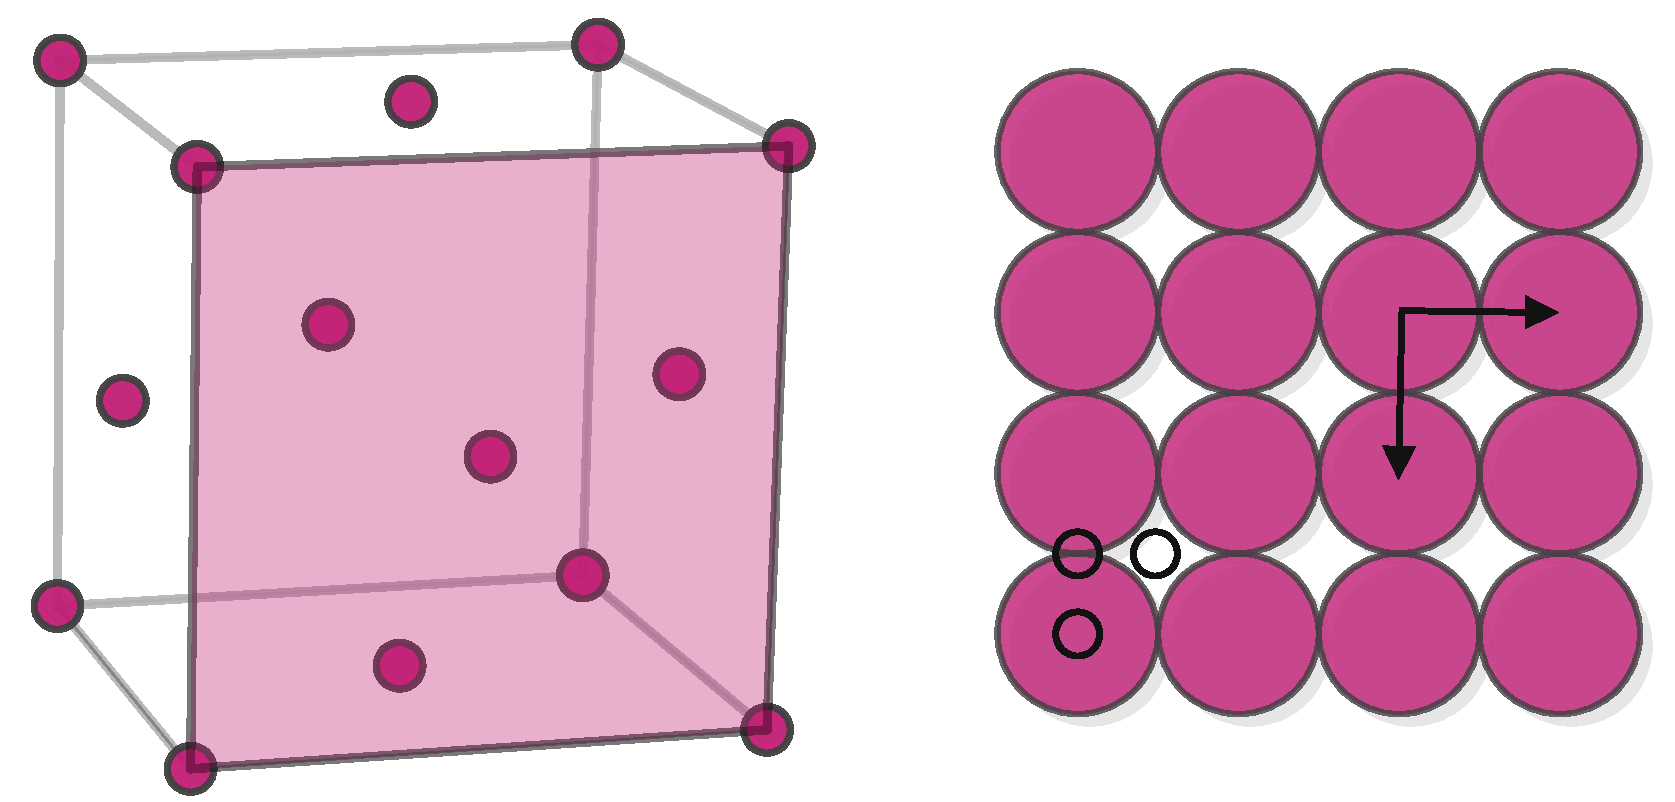
\includegraphics[width=0.9\textwidth]{images/vertiefer/Ag(100).pdf}
	\caption{Unit cell of the silver crystal with marked (100) plane and the Ag(100) surface with the unit cell vectors (black arrows) and the distinct adsorption sites (black circles).}
	\label{fig:Ag(100)}
\end{figure}

\ac{BE}

\newpage
\section{Experimental setup}

\begin{figure}[htbp]
	\centering
	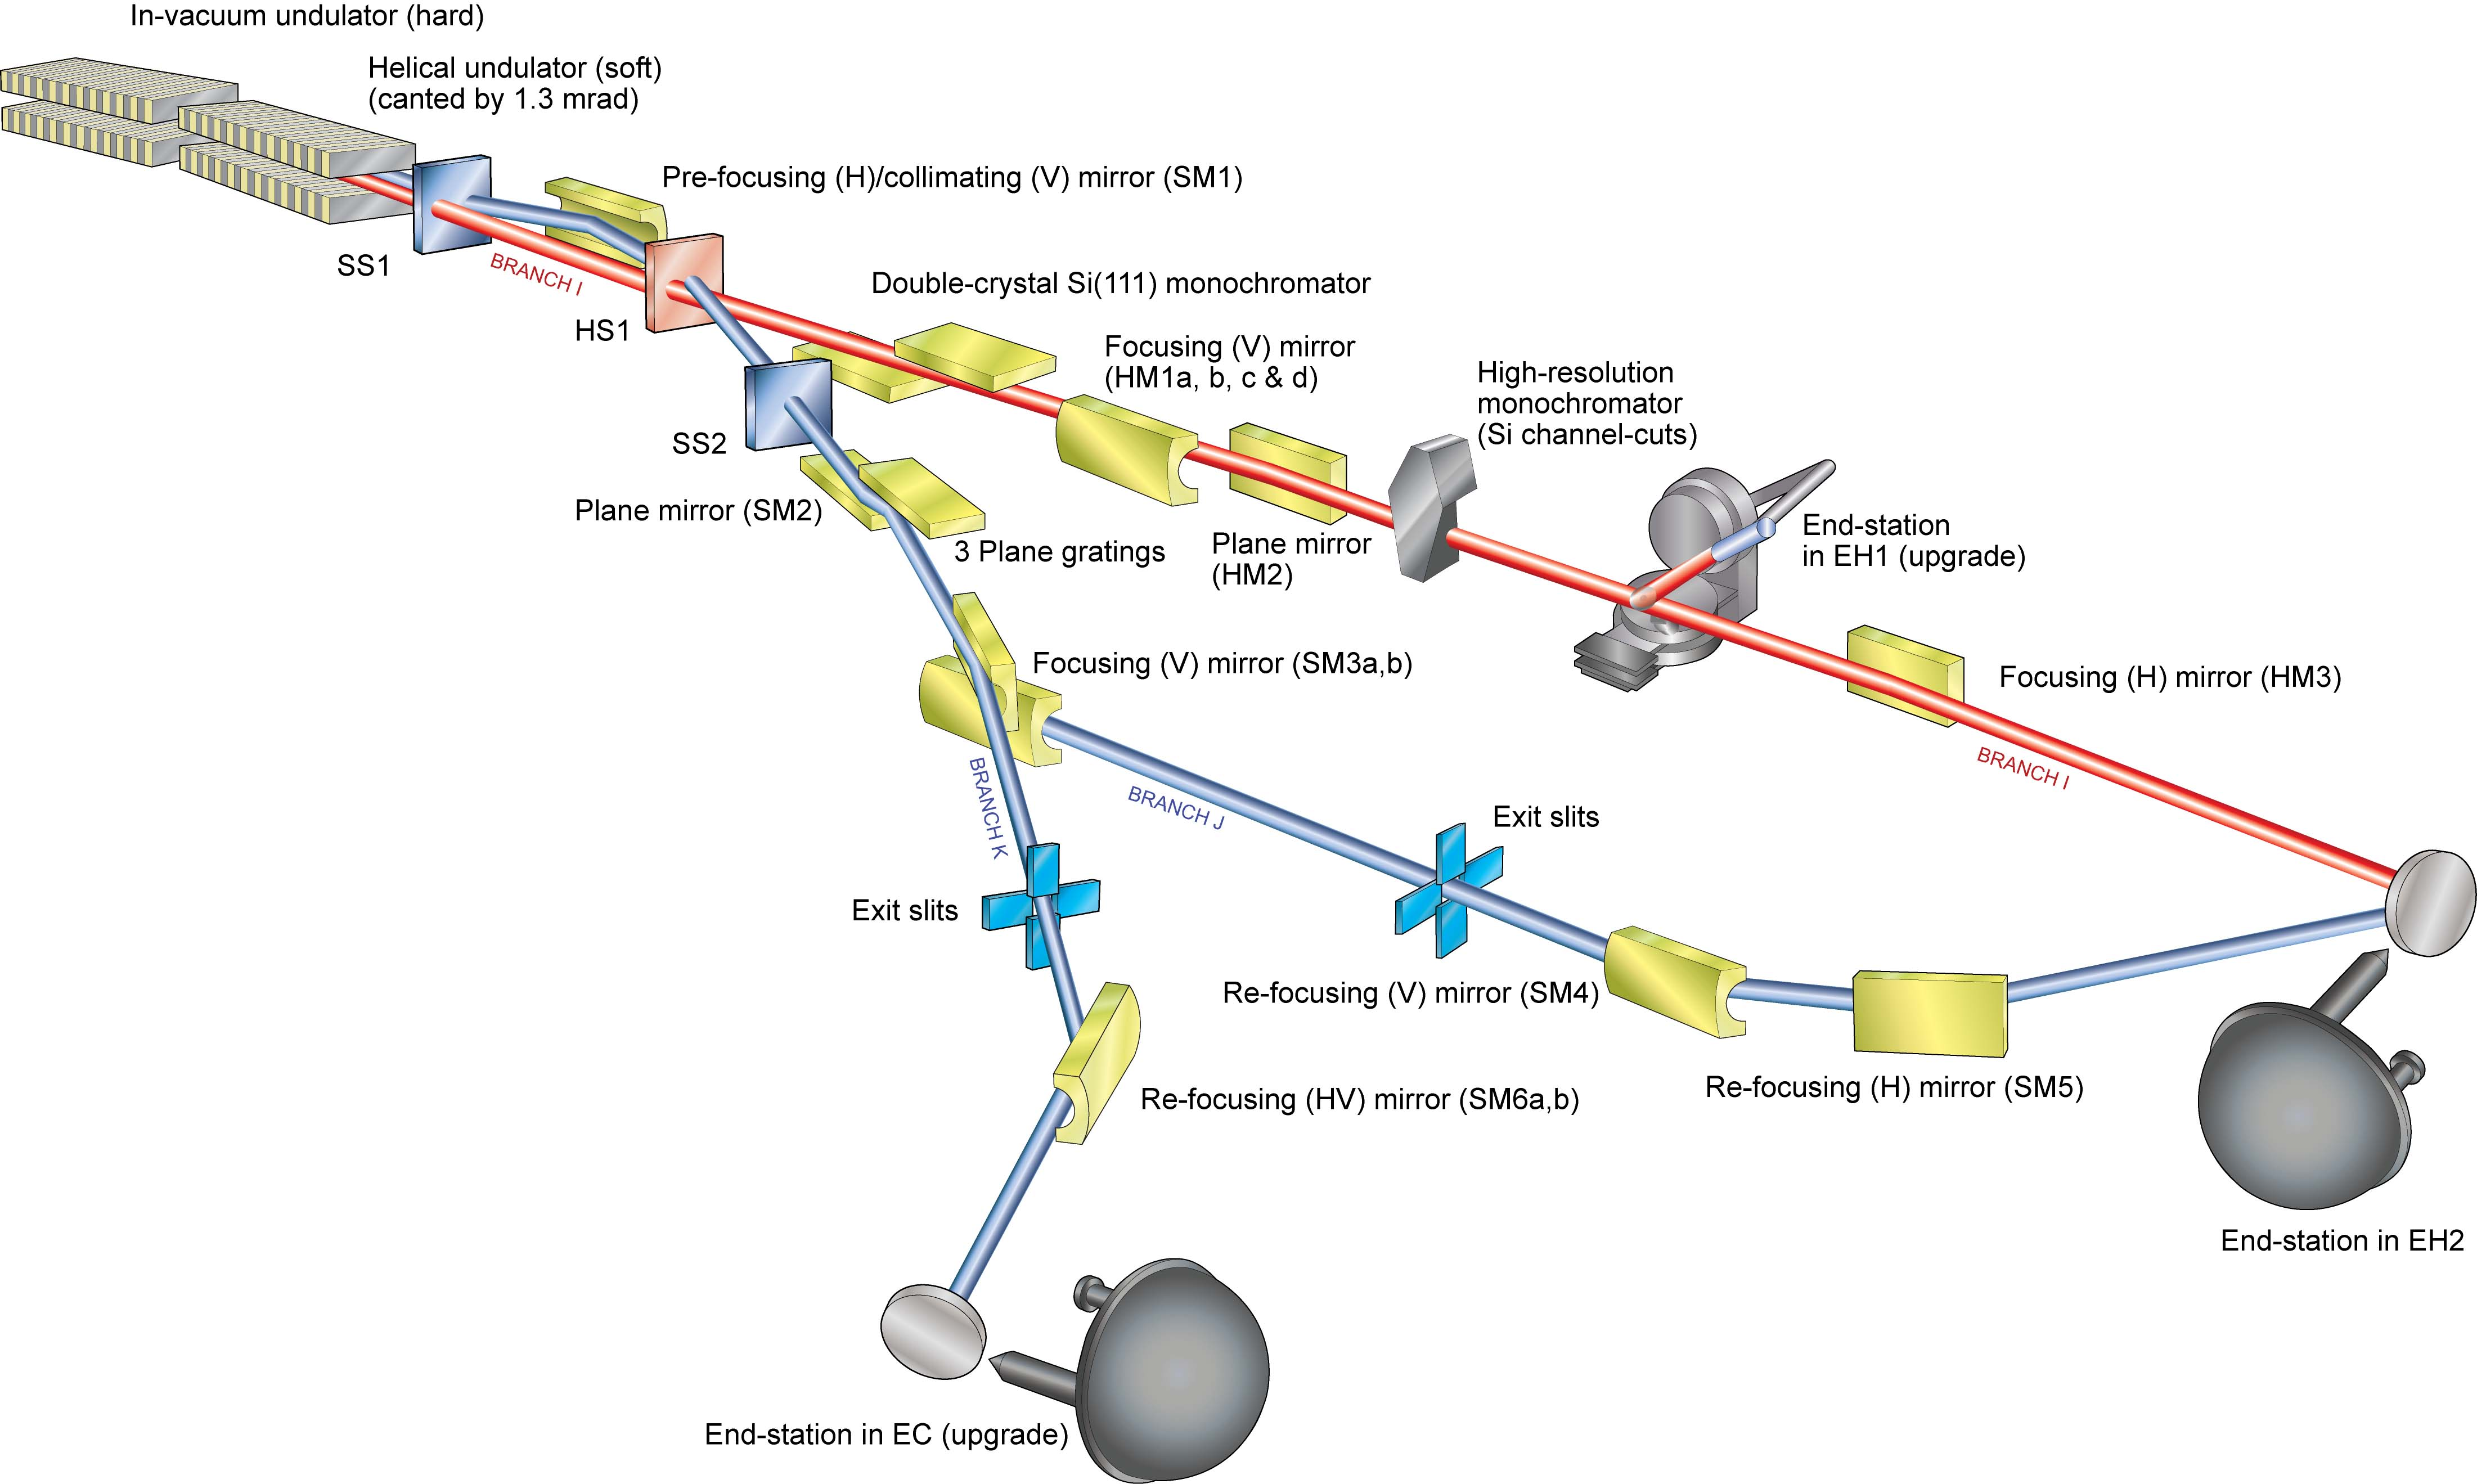
\includegraphics[width=0.9\textwidth]{images/vertiefer/I09.jpg}
	\caption{Schematic drawing of the I09 endstation of the Diamond Light Source in Didcot, UK. Picture taken from reference \cite{Diamond2025}.}
	\label{fig:I09}
\end{figure}

\begin{figure}[htbp]
	\centering
	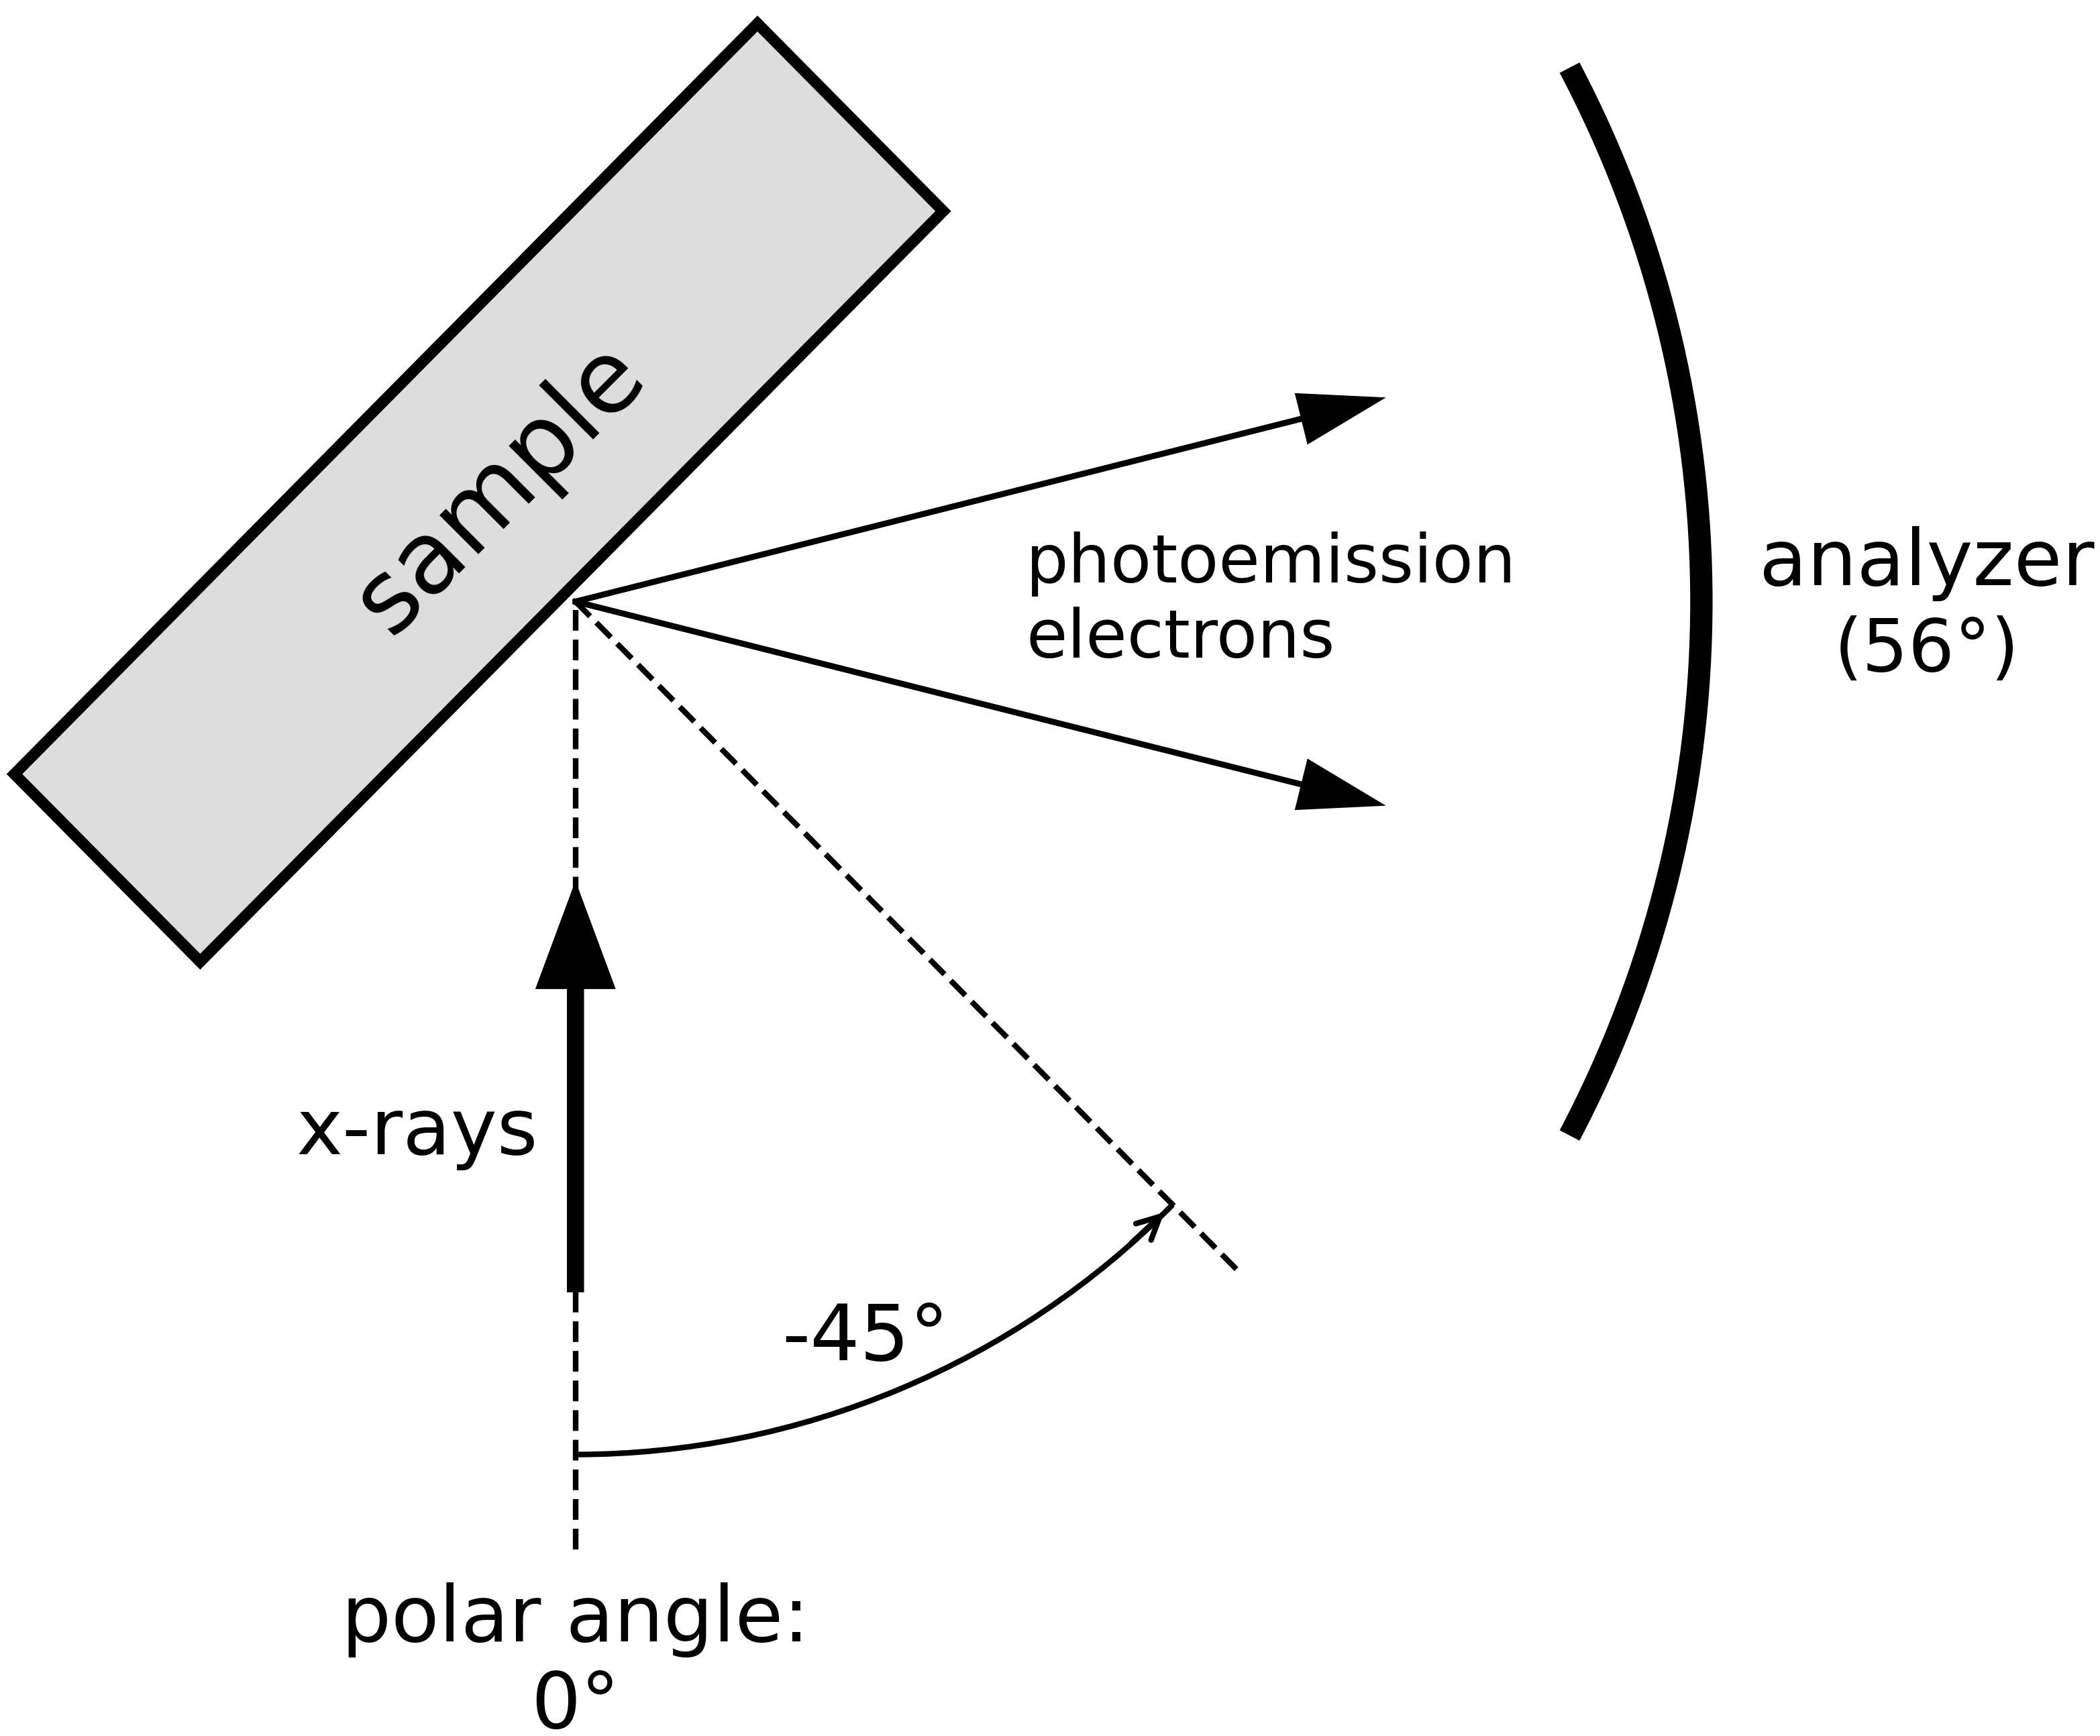
\includegraphics[width=0.6\textwidth]{images/vertiefer/experimental.png}
	\caption{Top view of the sample geometries for the \ac{XPS} measurements at the I09 endstation of the Diamond Light Source in Didcot, UK. Illustrated as in reference \cite{Kny2025}.}
	\label{fig:experimental}
\end{figure}

\begin{table}[H]
	\centering
	\caption{Experimental parameters for \ac{XPS} measurements at the I09 endstation of the Diamond Light Source in Didcot, UK.}
	\begin{tabular}{@{}ccccc@{}} \toprule
		& photon energy $E_\mathrm{\gamma}$ & pass energy $E_\mathrm{pass}$ & step width & number of frames \\
		\midrule
		C1s & 500~\si{\eV} & 20~\si{\eV} & 40~\si{meV} & 17 \\ 
		O1s & 630~\si{\eV} & 20~\si{\eV} & 40~\si{meV} & 17 \\ 
		N1s & 500~\si{\eV} & 20~\si{\eV} & 40~\si{meV} & 17 \\
		\bottomrule
	\end{tabular}
	\label{tab:experimental}
\end{table}

\section{Data processing}

\begin{table}[H]
	\centering
	\caption{Parameters used in CasaXPS\autocite{CasaSoftwareLtd2022} for the different peaks of the \ac{XPS} spectra of \ac{QA} on Ag(100).}
\begin{tabular}{@{}ccc@{}} \toprule
	~~~~~~peak~~~~~~ & ~~~~~~line shape~~~~~~ & ~~~~~~area ratio~~~~~~ \\
	\midrule
	$\mathrm{C_{arom}}$ & LA(1,8,800) & 10 \\
	$\mathrm{C_{NH}}$ & LA(1,8,800) & 4 \\
	$\mathrm{C_{CO}}$ & LA(1,8,800) & 4 \\
	$\mathrm{C_{O}}$ & LA(1,8,200) & 2 \\
	\midrule
	O1 & LA(1,8,400) & 1 (for $\beta$-phase) \\
	$\mathrm{O1_{sat}}$ & LA(1,1,400) & - \\
	O2 & LA(1,8,400) & 1 (for $\beta$-phase) \\
	$\mathrm{O2_{sat}}$  & LA(1,1,400) & - \\
	\midrule
	N1 & LA(1,8,400) & 1 (for $\beta$-phase) \\
	$\mathrm{N1_{damage}}$  & LA(1,8,400) & - \\
	N2 & LA(1,8,400) & 1 (for $\beta$-phase) \\
	\bottomrule
\end{tabular}
	\label{tab:casa}
\end{table}

\cleardoublepage
